\chapter{Cálculo de la constante $\mathcal{A}$ (Capítulo 2)} \label{apen:constante-A}

Como se menciona en el Capítulo \ref{cap:modelo}, la temperatura en la pared, promediada en el tiempo y en la dirección $Z$, crece linealmente con la coordenada $x$, esto es, $\langle T_w \rangle = \mathcal{A} \hspace{0.5mm} x $. Se procede entonces con el cálculo de la constante $\mathcal{A}$. Esto se realiza mediante un balance de energía en el dominio de simulación, es decir, $L_x \times L_y \times L_z$ (véase Figura \ref{fig:apendice-b}). 

\begin{figure}[H]
  \centering  
    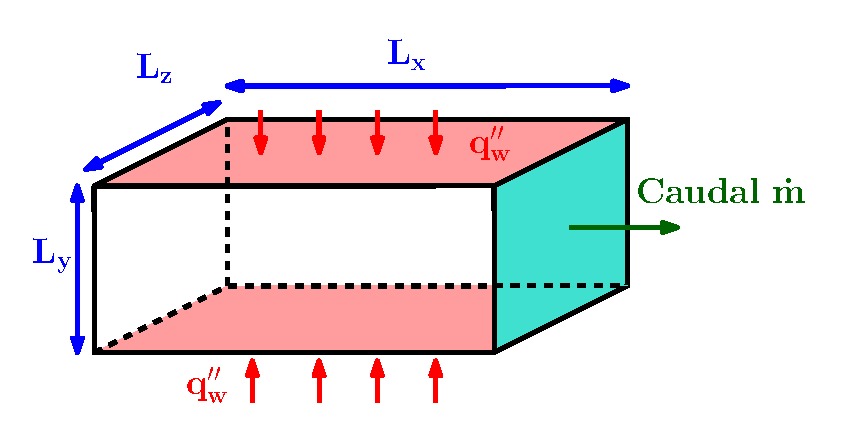
\includegraphics[width=0.6\textwidth]{figures/apendices/apendice_b.eps}
  \caption{Esquema del balance de energía.}
  \label{fig:apendice-b}
\end{figure}
De acuerdo con \cite{cengelheat}, dicho balance puede expresarse de la siguiente forma:

\begin{align*}
q'' S &= \int_A \rho \hspace{0.5mm} c_p \hspace{0.5mm} \left[ T_{out} - T_{in} \right] \hspace{0.5mm} (\mathbf{u} \cdot \mathbf{dA}) \\
	  &= c_p \hspace{0.5mm} \int_A \left[ T_{out} - T_{in} \right] \hspace{0.5mm} \rho \hspace{0.5mm} u_x \hspace{0.5mm} dA
\end{align*}
donde $q''$ es el flujo externo de calor, $S$ es el área de sección transversal al flujo de calor, $A$ es el área de sección transversal al flujo de masa, $c_p$ es el calor específico a presión constante, $T_{out}$ es la temperatura del fluido a la salida ($x=L_x$) y $T_{in}$ es la temperatura del fluido a la entrada ($x=0$). Considérese, por un lado, el cambio de variable realizado en la temperatura para satisfacer las condiciones de contorno periódicas (relaciones \ref{eq:pbc1} y \ref{eq:pbc2}), esto es, $T(x,y,z,t)= \langle T_w \rangle - \theta(x,y,z,t)$; y por el otro, que $T_{out}=T(x=L_x,y,z,t)$ y $T_{in}=T(x=0,y,z,t)$. Entonces, la diferencia de temperatura entre la entrada y la salida se puede escribir de la siguiente forma:

\begin{equation*}
\begin{aligned}
\left( T_{out} - T_{in} \right) &= T(x=L_x,y,z,t) - T(x=0,y,z,t) \\
								&= \left[ \mathcal{A} \hspace{0.5mm} L_x - \underbrace{\theta(x=L_x,y,z,t)}_{=0} \right] - \underbrace{ \left[ \mathcal{A} \hspace{0.5mm} 0 - \theta(x=0,y,z,t) \right] }_{=0} \\
								&= \mathcal{A} \hspace{0.5mm} L_x
\end{aligned}
\end{equation*}
Luego, si se tiene en cuenta que $q''= 2 q''_w$ y  $S=L_x L_z$ , al juntar todo lo anterior se encuentra que 
$$ 2 q''_w \hspace{0.5mm} L_z = c_p \hspace{0.5mm} \mathcal{A}  \hspace{0.5mm} \int_A  \rho \hspace{0.5mm} u_x \hspace{0.5mm} dA $$
Finalmente, tomando la aproximación de la integral como  $ \int_A \rho \hspace{0.5mm} u_x  \hspace{0.5mm} dA \simeq \rho_o \hspace{0.5mm} U_b \hspace{0.5mm} L_y \hspace{0.5mm} L_z$  (siendo $U_b$ la velocidad \textit{bulk} \cite{pope2001turbulent}) y recordando que $L_y = 2 d$, donde $d$ es el semiancho del canal, se obtiene la expresión buscada:

\begin{equation}
\mathcal{A}=\frac{q''_w}{\rho_o \hspace{0.5mm} c_p \hspace{0.5mm} U_b \hspace{0.5mm} d } \text{ .}
\end{equation}

